\documentclass[12pt,a4paper]{article}

\usepackage[T2A]{fontenc}
\usepackage[utf8]{inputenc}
\usepackage[russian,english]{babel}
\usepackage{indentfirst}
\usepackage{hyperref}
\usepackage{amsmath,amsthm,amstext,amssymb,amscd}
\usepackage{mathtools}
\usepackage{mathrsfs}
\usepackage{graphicx}
\usepackage{caption}
\usepackage{subcaption}


\title{Метод Рунге-Кутты \\ Задача №7.2.3}
\author{Игорь Степанов, ФРТК, 213}

\begin{document}

\maketitle
\hrulefill

\section{Постановка задачи} % (fold)
\label{sec:problem}

Для решения задачи Коши системы ОДУ используется численный метод Рунге-Кутты, заданный таблицей Бутчера. \par

\begin{align*}
	u’& =-5u + 3\cdot10^{-2}v + 2w,& u(0)& = 2,\\
	v’& =-800v,& v(0)& = 4,\\
	w’& =-u - 5\cdot10^{-3}v - 2w,& w(0)& = 6
\end{align*}

\begin{center}
	\begin{tabular}{ c | c c }
		$1/6$ & $1/6$ & 0 \\
		$5/6$ & $4/6$ & $1/6$ \\ \hline
		& $1/2$ & $1/2$ \\
	\end{tabular}
\end{center} \par
Получить для него функцию и условие устойчивости. Вычислите число жесткости. \par

% section problem (end)

\section{Выкладки} % (fold)
\label{sec:theory}

\subsection{Функция устойчисвости} % (fold)
\label{sub:stability}

Функция устойчивости имеет вид:
\begin{equation}
	R(z) = 1 + z \overrightarrow{b}^{tr}({\bf E} - z {\bf A})^{-1}\overrightarrow{1}.
\end{equation} \par
Аналитически приводим эту функцию к виду:
\begin{equation}
	R(z) = \dfrac{1 + z - \frac{5}{36} z^2}{(1 - \frac{z}{6})^2}.
\end{equation} \par

Решение неравенства $\left| R(z) \right| \le 1$ представляет из себя 
$$ z \in \left[3(1-\sqrt{3}); 0 \right] \bigcup \left[8;3(1+\sqrt{3}) \right]. $$
Следовательно для шага $h$ получаем такое условие: 
$$ h \in \left(0; \frac{3(1-\sqrt{3})}{\lambda_{min}}\right] \simeq \left(0; 2.745 \cdot 10^{-3} \right]. $$

% subsection stability (end)

\subsection{Число жесткости} % (fold)
\label{sub:stiffness}

Для нахождения числа жесткости {\bf S} необходимо вычислить собственные числа матрицы Якоби: \\
\begin{equation*}
	{\bf Y} = 
	\begin{pmatrix}
	-5 & 3\cdot10^{-2} & 2 \\
	0 & -800 & 0 \\
	-1 & -5\cdot10^{-3} & -2
	\end{pmatrix}
\end{equation*} \par

Получаем: ${\lambda} {\in} \{-3, -4, -800\} $.
Число жесткости рассчитывается:
\begin{equation}
	S = \dfrac{|\lambda|_{max}}{|\lambda|_{min}} = \dfrac{800}{3} = 266.6(66)
\end{equation} \par

% subsection stiffness (end)

\subsection{Метод Рунге-Кутты} % (fold)
\label{sub:runge}

\begin{equation}
	\overrightarrow{u_{n+1}} = \overrightarrow{u_n} + h \sum_{i=1}^s b_i \overrightarrow{k_i},
\end{equation}
где
\begin{equation}
	\overrightarrow{k_i} = f\left(x_n + c_ih, \overrightarrow{u_n} + \sum_{j=1}^s a_{ij}k_j\right), i = \overline{1, s}, s = 2.
\end{equation}

\subsubsection{Явный метод Рунге-Кутты}
\label{ssub:explicit-runge}

\begin{equation} \label{eq:runge-x2}
	\overrightarrow{u_{n+1}} = \overrightarrow{u_n} + \frac{h}{2} \left( 3 \overrightarrow{f_n} - \overrightarrow{f_{n-1}} \right)
\end{equation}

На Рис.~\ref{fig:fig2} показано решение исходной задачи (раздел~\ref{sec:problem}) двухстадийным явным методом Рунге-Кутты (формула \ref{eq:runge-x2}). Сравнивая с Рис.~\ref{fig:fig1}, видно, что решения практически повторяют друг друга, а так как среде Matlab можно доверять, то и наше решение будет верным. \par
При уменьшении шага примерно до $h \simeq 0.1 $ двухстадийный метод становится непригодным для использования, а Matlab продолжает считать верно. \par

\begin{figure}
    \centering
    \begin{subfigure}[b]{\textwidth}
        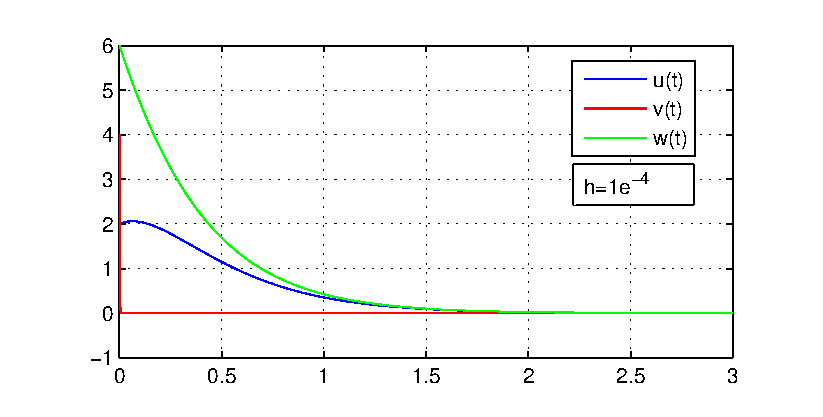
\includegraphics{runge-matlab.eps}
        \caption{Решение задачи, используя встроенный метод Рунге-Кутты в среде Matlab}
        \label{fig:fig1}
    \end{subfigure}
    \begin{subfigure}[b]{\textwidth}
        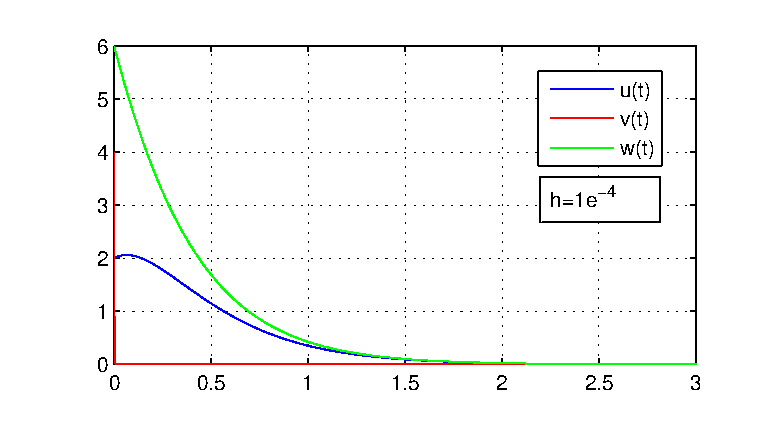
\includegraphics{runge-2x.eps}
        \caption{Решение задачи, используя двухстадийный явный метод Рунге-Кутты}
        \label{fig:fig2}
    \end{subfigure}
    \caption{Решения задачи}\label{fig:graph}
\end{figure}

% subsection runge (end)

% section theory (end)

\section{Заключение} % (fold)
\label{sec:summary}

Решить задачу указанным методом не получилось, т.к. коэффициенты преобретают слишком большие степени десяти, что приводит к переполнению стека программы. Так в {\bf Matlab} результат даже после первой итерации получается {\it Inf}. При этом это происходит при любом начальном приближении коэффициентов. \par
Возможно это из-за того, что в условии не надо было решать саму задачу Коши, а только лишь найти функцию устойчивости и число жесткости. Однако получилось найти решение используя двухстадийный явный метод. \par

% section summary (end)

\end{document}
